\documentclass[twocolumn,
			   showpacs,%
               nofootinbib,
               aps,%
               %eqsecnum,
               prd,
               notitlepage,
               showkeys,
               10pt]{revtex4-1}
               
%Loading my personal settings
\usepackage{todonotes}

%math and formulas
\usepackage{amssymb}
\usepackage{amsmath}
\usepackage{physics}

%language settings and microtype
\usepackage[english]{babel}
\usepackage{microtype}

%useful packages
\usepackage{graphicx}
\usepackage{siunitx}
\usepackage{xcolor}
\usepackage{float}
\usepackage{dcolumn}
\usepackage{blindtext}
\usepackage{xfrac}
\usepackage[labelfont=bf]{caption}
\usepackage{subcaption}


%feynman diagrams
\usepackage{tikz}
\usepackage{tikz-feynman}
\tikzfeynmanset{compat=1.0.0} 

%loading the `external` library
\usetikzlibrary{external}   
%Create directory to store the diagrams and all related files          
\immediate\write18{mkdir -p feynman-diagrams} 
% Activate externalization
\tikzexternalize[
  %Avoid cluttering the directory                     
  prefix=feynman-diagrams/, 
  %Calling lualatex externally
  system call={             
    lualatex \tikzexternalcheckshellescape -halt-on-error -interaction=batchmode -jobname="\image" "\texsource"  || rm "\image.pdf"
  },
]

%color settings
\definecolor{mydarkblue}{RGB}{1,1,141}

%correcting parindent
\setlength{\parindent}{0pt}


%always use hyperref at the end of the preamble!
\usepackage[colorlinks=True]{hyperref}
\hypersetup{allcolors=mydarkblue}
%main document
\begin{document}

%Personel data
{\hypersetup{allcolors=black}
\title{F91: Studying the $Z$ boson with the ATLAS Detector at the LHC }
\author{Mathieu Kaltschmidt}
\email{M.Kaltschmidt@stud.uni-heidelberg.de}
\affiliation{Heidelberg University,  D-69117 Heidelberg, Germany}
\author{Quirinus Schwarzenb\"ock}
\email{Schwarzenb\"ock@stud.uni-heidelberg.de}
\affiliation{Heidelberg University,  D-69117 Heidelberg, Germany}

\date[Carried out in the week of  ]{March 4$^{\text{th}}$, 2019}


\begin{abstract}
This experiment was performed as part of the advanced lab course for physics students (FP) at Heidelberg University.
The goal of this computer-based experiment is to determine the invariant mass spectrum for the $Z$ boson, one of the three massive gauge bosons of the weak interaction, using data acquired by the ATLAS experiment at the Large Hadron Collider (LHC) at CERN in Geneva. For data-analysis  and plotting we used \verb|ROOT| and different \verb|Python| scripts.
\end{abstract}

\maketitle


}
\section{Introduction}
In this lab course about the $Z$ boson, we want to study its properties and get familiar with modern data analysis tools such as \verb|ROOT| and \verb|Python3|, used in current experimental high-energy physics research. The data we used, is part of the ATLAS Open Data set, published by CERN to provide students a hands-on training experience for data analysis. It features real data from the LHC measured in 2012 and additionally some Monte-Carlo simulations of the same processes for a better comparability with the theoretical predictions.

\subsection{The $Z$ boson}
In this section, we want to introduce the theoretical properties of the $Z$ boson. The most important are summarized in the following:

\begin{table}[!htbp]
	\centering
	\renewcommand{\arraystretch}{1.5}
	\begin{tabular}{c|c|c|c}
	Charge $Q$ & Spin $S$ & Mass $M_Z$ [GeV] & Decay Width $\Gamma$ [GeV] \\ \hline 
	 0 & 1 & $(91.1876 \pm 0.0021)$ & $(2.4952 \pm 0.0023)$ \\
		\end{tabular}
	\caption{\label{tab:Z_props}The properties of the $Z$ boson.}
\end{table}

The $Z$ boson is one of the three gauge bosons of the weak interaction. In contrast to photons, which mediate the electromagnetic force, or gluons, the gauge bosons of the strong interaction, it is massive. It has two charged "cousins", the $W^+$ and the $W^-$ boson. Postulated by Glashow, Salam and Weinberg in the 1960s as part of the unified electroweak interaction, which earned them a Nobel prize in 1979, it has not been directly observed until 1983, at the SPS collider at CERN, when particle colliders were able to reach center-of-mass energies high enough. The detection of the $Z$ earned Carlo Rubbia and Simon van der Meer also a Nobel prize in 1984.   


\section{Theoretical Foundations}
This section introduces the basic knowledge on particle and detector physics needed for a general understanding of the conducted experiment.

\subsection{Drell-Yan processes}
Hadrons, i.\,e. particles made up of three quarks, scattering at very high energies can decay in so called Drell-Yan processes, which play an important role in high energy particle collisions. These occur, when a quark and its corresponding antiquark annihilate each other via a virtual boson, for example a $Z$, we are interested in in this lab course. A Feynman diagram for a simple Drell-Yan process is depicted in the following in figure (\ref{fig:Drell-Yan}).

\begin{figure}[H]
\centering
\feynmandiagram [small] [horizontal' = a to b] {
	i1 [particle=\(q\)] -- [fermion] a  -- [fermion] i2 [particle=\(\overline{q}\)],
	a -- [photon, edge label=\(\gamma / Z^0\)] b ,
	f1 [particle=\(l^{+}\)] -- [fermion] b -- [fermion] f2 [particle=\(l^{-}\)],
	};
\caption{A simple Drell-Yan diagram, inspired by \cite{F91manual}}
\label{fig:Drell-Yan}
\end{figure}
	
To study the properties of the boson involved in these processes one can calculate for example the invariant mass $\sqrt{s}$, using the following formula:
\begin{align}
	\sqrt{s} = \sqrt{\left(p_{l^{-}} + p_{l^{+}}\right)^2}
\end{align}
We will see later on, how this formula can be used to discard useless data.
\subsection{Characteristics of Particle Detectors}
In circular particle colliders such as the LHC, two opposed proton beams, each containing $n_b = 1380$ bunches with approximately $N_i = 1011$ protons are accelerated to almost the speed of light and forced to collide at very high center-of-mass energies, e.\,g. $\sqrt{s} = 8$ TeV in the first run of the LHC. An important characteristic of circular colliders is the \textit{luminosity} $\mathcal{L}$, given by

\begin{align}
\mathcal{L} = \frac{N_1N_2f_{\text{rev}}n_b}{4\pi\sigma_x\sigma_y}
\end{align}
where $f = 11.2$ kHz describes the orbital frequency of the beams and the $\sigma_i$ describe the smearing of the beam in the respective direction. At the LHC, they reach luminosities of $\mathcal{L}=10^{34} \ \mathrm{cm}^{-2} \mathrm{s}^{-1}$.\\
To obtain the entire information content of the events one can integrate the luminosity over time to get the \textit{integrated luminosity}:
\begin{align}
\mathcal{L}_{\text{int}} = \int \mathcal{L} \ \dd t.
\end{align}
The data we are analyzing has an integrated luminosity of $\mathcal{L}_{\mathrm{int}}=1 \ \mathrm{fb}^{-1}$.\\
Together with the \textit{total cross section} $\sigma_{pp\rightarrow X}$ one finds the following relation for the rate of events $N$: 
\begin{align}
N = \sigma_{pp\rightarrow X} \cdot \mathcal{L}_{\text{int}}.
\end{align}

\subsection{Energy distributions}
\textbf{Gaussian distribution.} Inside the calorimeter, the energies are distributed following a \textit{Gaussian}, i.\,e. 
\begin{align}
g(E ; \mu, \sigma)=\frac{\mathcal{N}}{\sqrt{2 \pi} \sigma} \exp \left[-\frac{(E-\mu)^{2}}{2 \sigma^{2}}\right]
\label{eqn:Gaussian}
\end{align}
with an arbitrary normalization constant $\mathcal{N}$. The important parameter in this distribution is the standard deviation $\sigma$ which allows us to estimate the uncertainty of the energy.\\

\textbf{Breit-Wigner distribution.} The physical decay process is described by the \textit{Relativistic Breit-Wigner distribution}, 
\begin{align}
	f(E ; M, \Gamma)=\frac{\mathcal{N} k}{\left(E^{2}-M^{2}\right)^{2}+M^{2} \Gamma^{2}}
\end{align}
where $k=\frac{2 \sqrt{2} M \Gamma \gamma}{\pi \sqrt{M^{2}+\gamma}}$ and $\gamma=M \sqrt{M^{2}+\Gamma^{2}}$. The parameter $M$ represents the mass and $\Gamma$ is the decay width of the observed process. For a derivation see for example \cite{BohmSato2004}. \\

In order to describe the real measured process we have to convolute a Breit-Wigner distribution and a Gaussian. This takes the smearing of the curve due to uncertainties in the measure electronics into account which are described by the Gaussian (\ref{eqn:Gaussian}). \\

The convolution of both distributions leads us the so called, \textit{Relativistic Voigt Profile}
\begin{align}
	V(E ; M, \Gamma, \sigma)=\int \mathrm{d} E^{\prime} g\left(E^{\prime} ; 0, \sigma\right) f\left(E-E^{\prime} ; M, \Gamma\right).
\end{align}
We will use this function later on to fit the filtered data set. A comparison to the fits with the two single distributions is also included. 
\subsection{The ATLAS Detector at the LHC}

Three major components form the setup of the ATLAS detector, i.\,e. the \textit{Inner Detector}, which aims at reconstructing the tracks of charged particles passing the detector, the \textit{Calorimeter}, where the electromagnetic and hadronic showers are evaluated and the \textit{Muon Spectrometer} in the outer layer, to reconstruct muon tracks, which have in general a free path length much longer than the other charged particles occurring in this processes. Additionally there is complex \textit{Trigger System} to avoid the collection of irrelevant data and the so called \textit{GRID}, a web-based network to make the measured data accessible to the world-wide particle physics community working on ATLAS physics. \\
A schematic overview is presented in figure (\ref{fig:atlas}) in the following.
\begin{figure}[H]
\centering
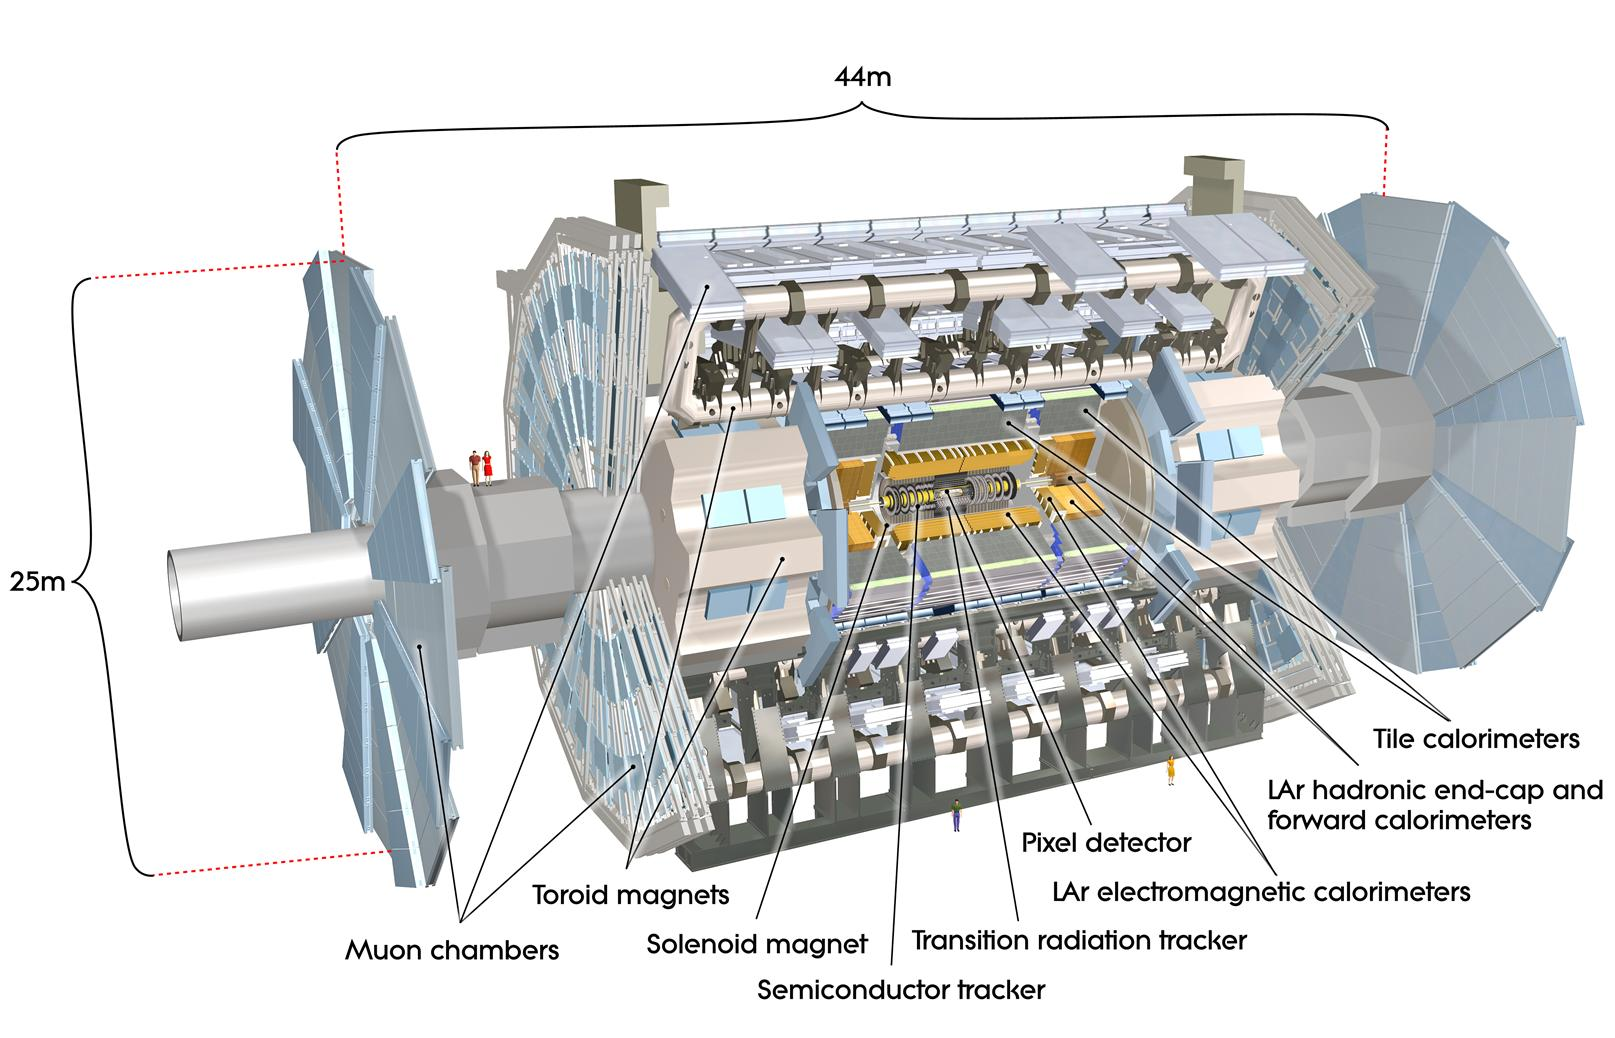
\includegraphics[width=0.45\textwidth]{figures/introduction/atlas}
\caption[Schematic picture of the ATLAS detector at the LHC.]{Schematic picture of the ATLAS detector at the Large Hadron Collider\footnotemark.}
\label{fig:atlas}
\end{figure}
\footnotetext{Picture taken from \url{http://www.kip.uni-heidelberg.de/kw/image/f/group/f8/webutils/atlas.jpeg} (\tiny{\today})}
\subsection{Detector Geometry}
An important quantity for the understanding the geometry of particle detectors is the \textit{pseudorapidity} $\eta$, which is used to describe polar angle distributions, i.\,e.
\begin{align}
\eta = -\ln \tan(\frac{\theta}{2}).	\label{eqn:eta}
\end{align}

From the geometry of the setup it is easy to find the following relations between the momentum components $p_i$ and transversal momentum $p_T$:
\begin{align}
	p_x &= p_T \cos(\phi)\\
	p_y &= p_T \sin(\phi)\\
	p_z \tan(\theta) &= p_T
\end{align}
From equation (\ref{eqn:eta}) and with the help of the identity
\begin{align*}
\tan(2\arctan(x)) = \frac{2x}{1 - x^2},
\end{align*} 
we arrive at the following formulas:
\begin{align}
	p_z &= p_T\sinh(\eta)\\
	\left|\mathbf{p}\right| &= p_T \cosh(\eta).
\end{align}


\subsection{Efficiency of the measurements}
This section describes the so called \textit{tag and probe method}, which allows us to determine the unbiased efficiency of the measurement and filtering process.\\
One of the two electrons (the \textit{tag} electron) has to pass very strong selection criteria. The next step is to check wether the second electron (the \textit{probe}) passes the slightly less strict criteria, which are explained in more detail later on, when we discuss the implementation of the multi-level filter system. \\
Then, the last step is to determine the efficiency $\epsilon$ by calculating the ratio between the successful passing probe electrons and the total amount of probes.\\
For the \textit{total efficiency} $\epsilon_{\text{tot}}$ we find 
\begin{align}
	\epsilon_{\text{tot}} = \epsilon_{\text{reconstr.}} \cdot \epsilon_{\text{ident.}} \cdot \epsilon_{\text{trigger}} \cdot \epsilon_{\text{add.}},
\end{align}
 where the additional efficiencies come from the other filter steps, e.\,g. the isolation values. 

\begin{figure}[H]
\centering
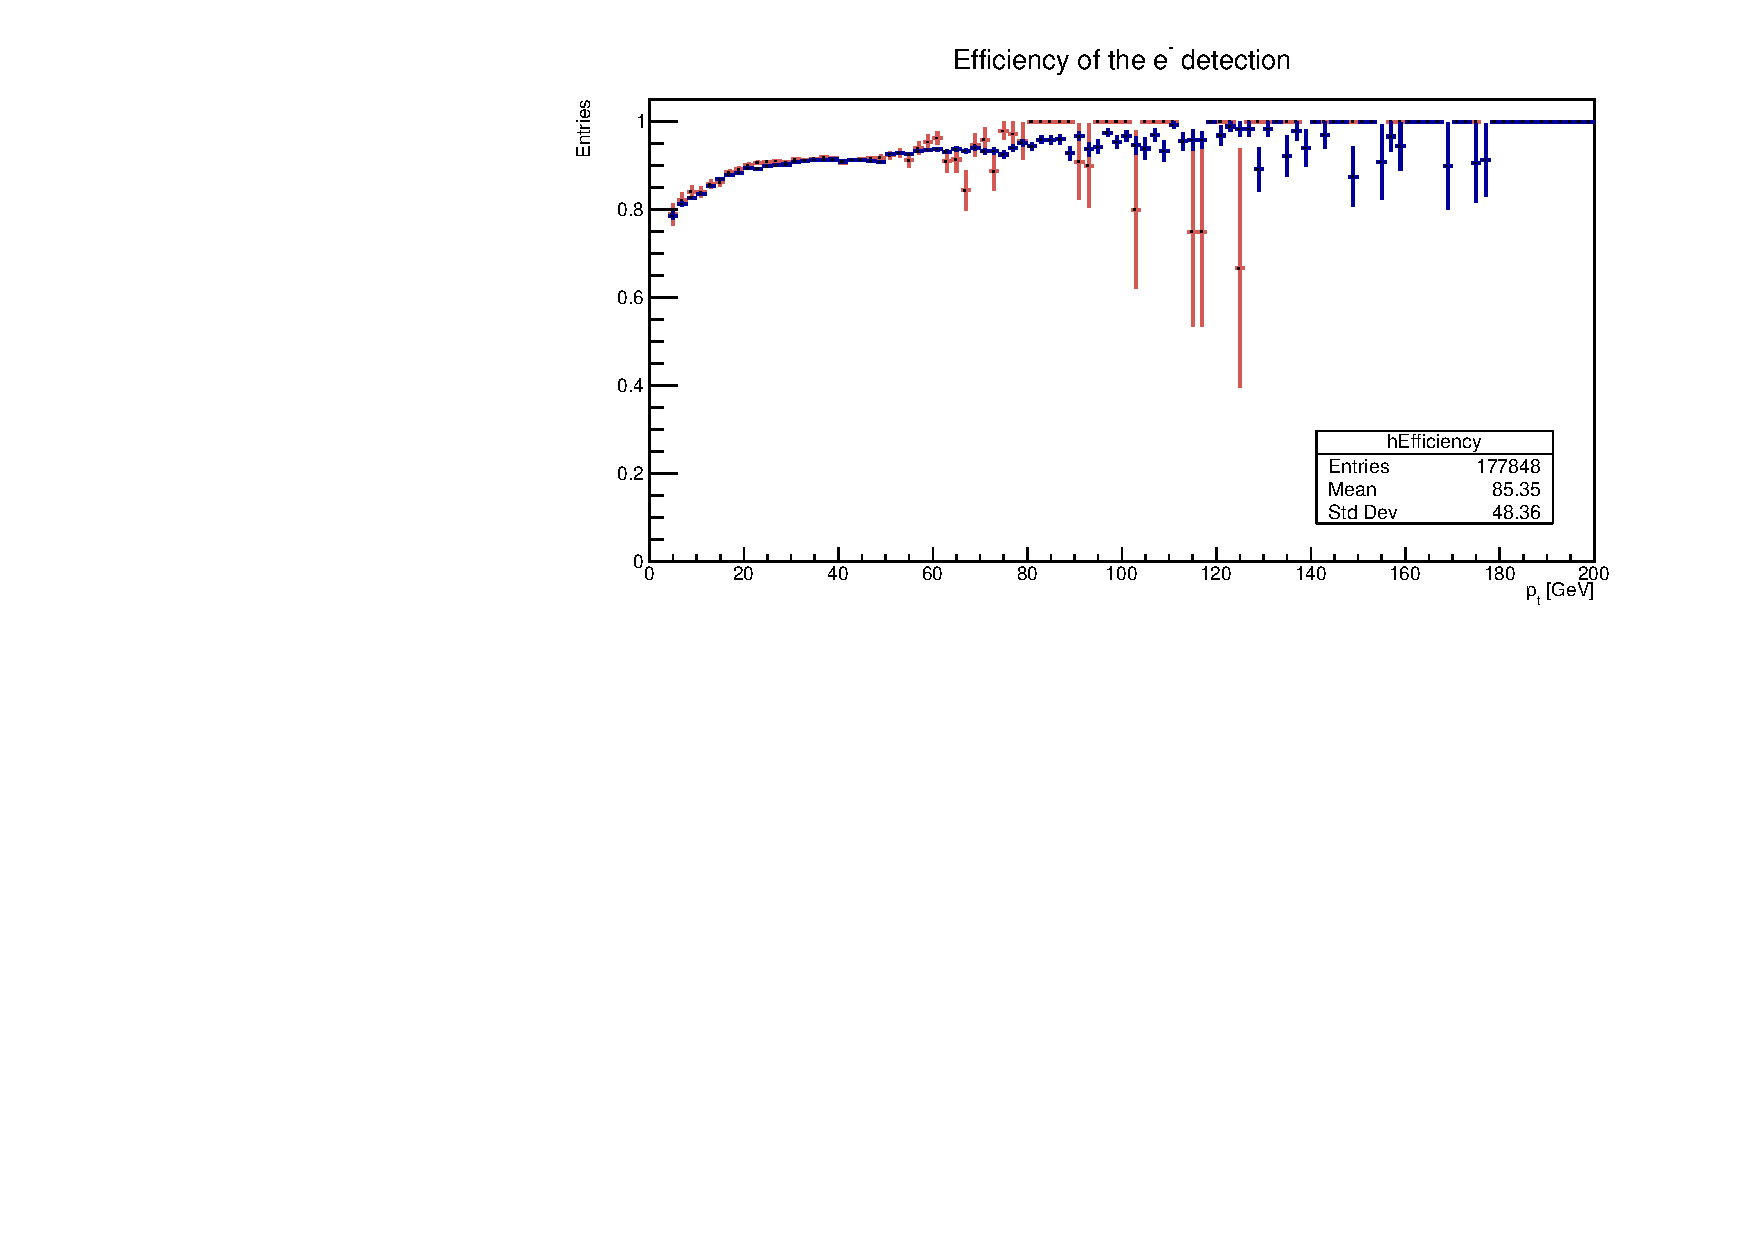
\includegraphics[width=0.45\textwidth]{figures/plots/efficiency}
\caption{Efficiency measurement for the real data (red) and the MC simulations (blue).}
\end{figure}
%TODO: Rot=exp , Blau=MC
\section{Experiment}

Having to learn the basics of \verb|ROOT| and to get familiar with the dataset, we start with some simple plots giving us already some information about the most important characteristics of the conducted measurements.\\

\textbf{Primary Vortices.} The first diagram displays the distribution of the primary vertices along the $z$-direction after a collision of two bunches.
\begin{figure}[H]
\centering
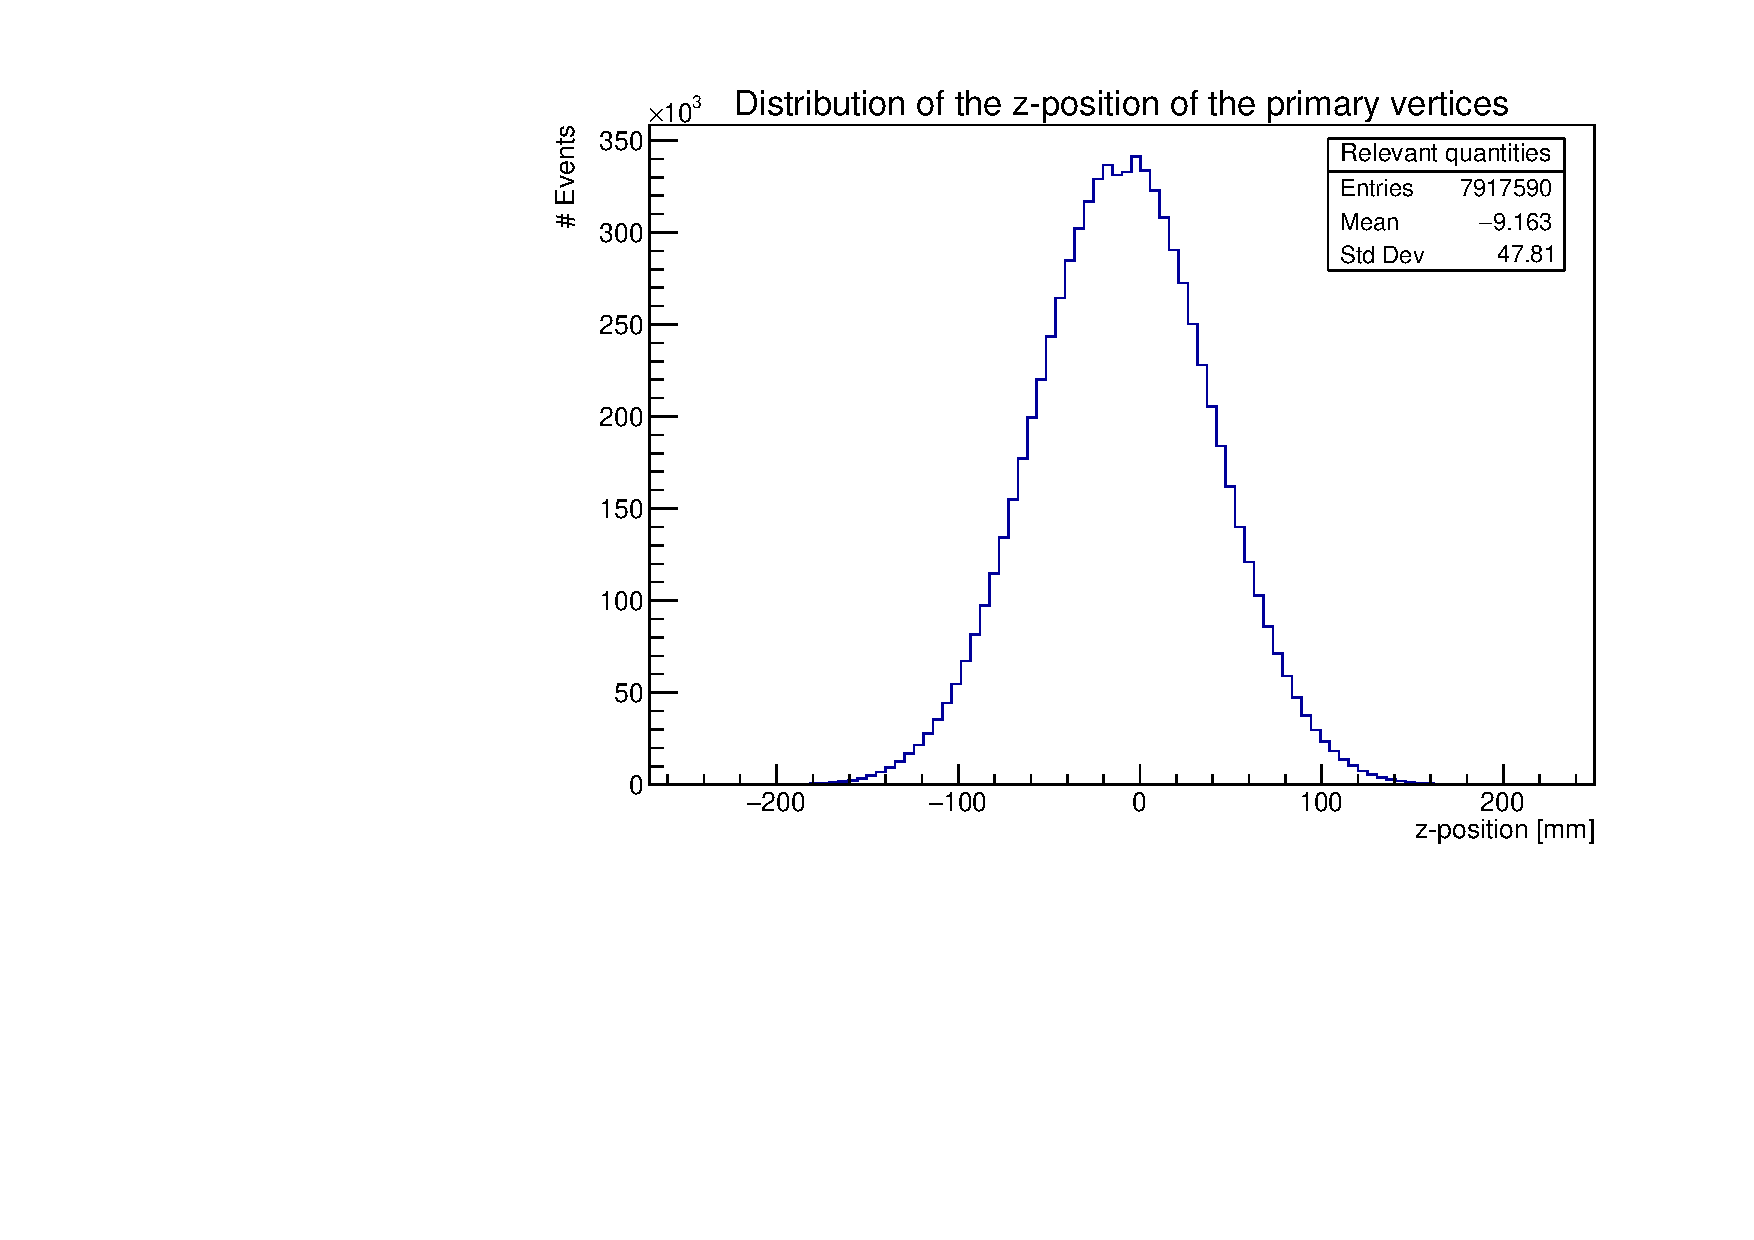
\includegraphics[width = 0.45\textwidth]{figures/plots/DistPrimVort}
\caption{Distribution of the primary vortices.}
\label{fig:vortices}
\end{figure}
The distribution depicted in figure (\ref{fig:vortices}) is explained by the fact, that the bunches are spread along the $z$-axis, which makes it impossible for all collisions to happen at the same $z$-coordinate.\\

\textbf{Lepton Number.} It is very likely for two-quark decay-processes to end up in one-, two- or three-lepton final states. \footnote{Neutrinos are neglected in this consideration, since they are very hard to detect and should have little to no noticeable effect on our results.} The following Feynman diagrams represent some of the constellations mentioned above. 

\begin{figure}[H]
\centering	
\feynmandiagram [small] [horizontal' = a to b] {
	i1 [particle=\(\overline{u}\)] -- [fermion] a  -- [fermion] i2 [particle=\(d\)],
	a -- [photon, edge label=\(W^{-}\)] b ,
	f1 [particle=\(\nu_{e^{-}}\)] -- [fermion] b -- [fermion] f2 [particle=\(e^{-}\)],
	};
\caption{1-Lepton final state.}
\end{figure}

\begin{figure}[H]
\centering	
\feynmandiagram [small] [horizontal' = a to b] {
	i1 [particle=\(q\)] -- [fermion] a  -- [fermion] i2 [particle=\(\overline{q}\)],
	a -- [photon, edge label=\(\gamma / Z^0\)] b ,
	f1 [particle=\(e^{+}\)] -- [fermion] b -- [fermion] f2 [particle=\(e^{-}\)],
	};
\caption{2-Lepton final state.}
\end{figure}

\begin{figure}[H]
\centering	
\begin{tikzpicture}
  \begin{feynman}
    \vertex (a) {\(d\)};
    \vertex [right=of a] (b);
    \vertex [above right=of b] (c);
    \vertex [above right=of c] (f1) {\(e^{-}\)};
    \vertex [below right=of c] (f2) {\(\overline{\nu}_{e^{-}}\)};
    \vertex [below =of a] (d) {\(\overline{u}\)};
    \vertex [right=of d] (e);
    \vertex [below right=of e] (f);
     \vertex [above right=of f] (f3) {\(e^{-}\)};
    \vertex [below right=of f] (f4) {\(e^{+}\)};

 
    \diagram* {
      (a) -- [fermion] (b) -- [boson, edge label=\(W^{-}\)] (c),
      (d) -- [anti fermion] (e) -- [boson, edge label'=\(Z^{0}\)] (f),
      (f1) -- [anti fermion] (c) -- [anti fermion] (f2),
      (f3) -- [anti fermion] (f) -- [anti fermion] (f4),
      
      (b) -- [edge label' = \(\overline{u}\) ] (e),
};
  \end{feynman}
\end{tikzpicture}
\caption{3-Lepton final state.}
\end{figure}

To check this, we plot the amount of lepton candidates in the final state for our dataset. The result is presented in the following figure.

\begin{figure}[H]
	\centering
	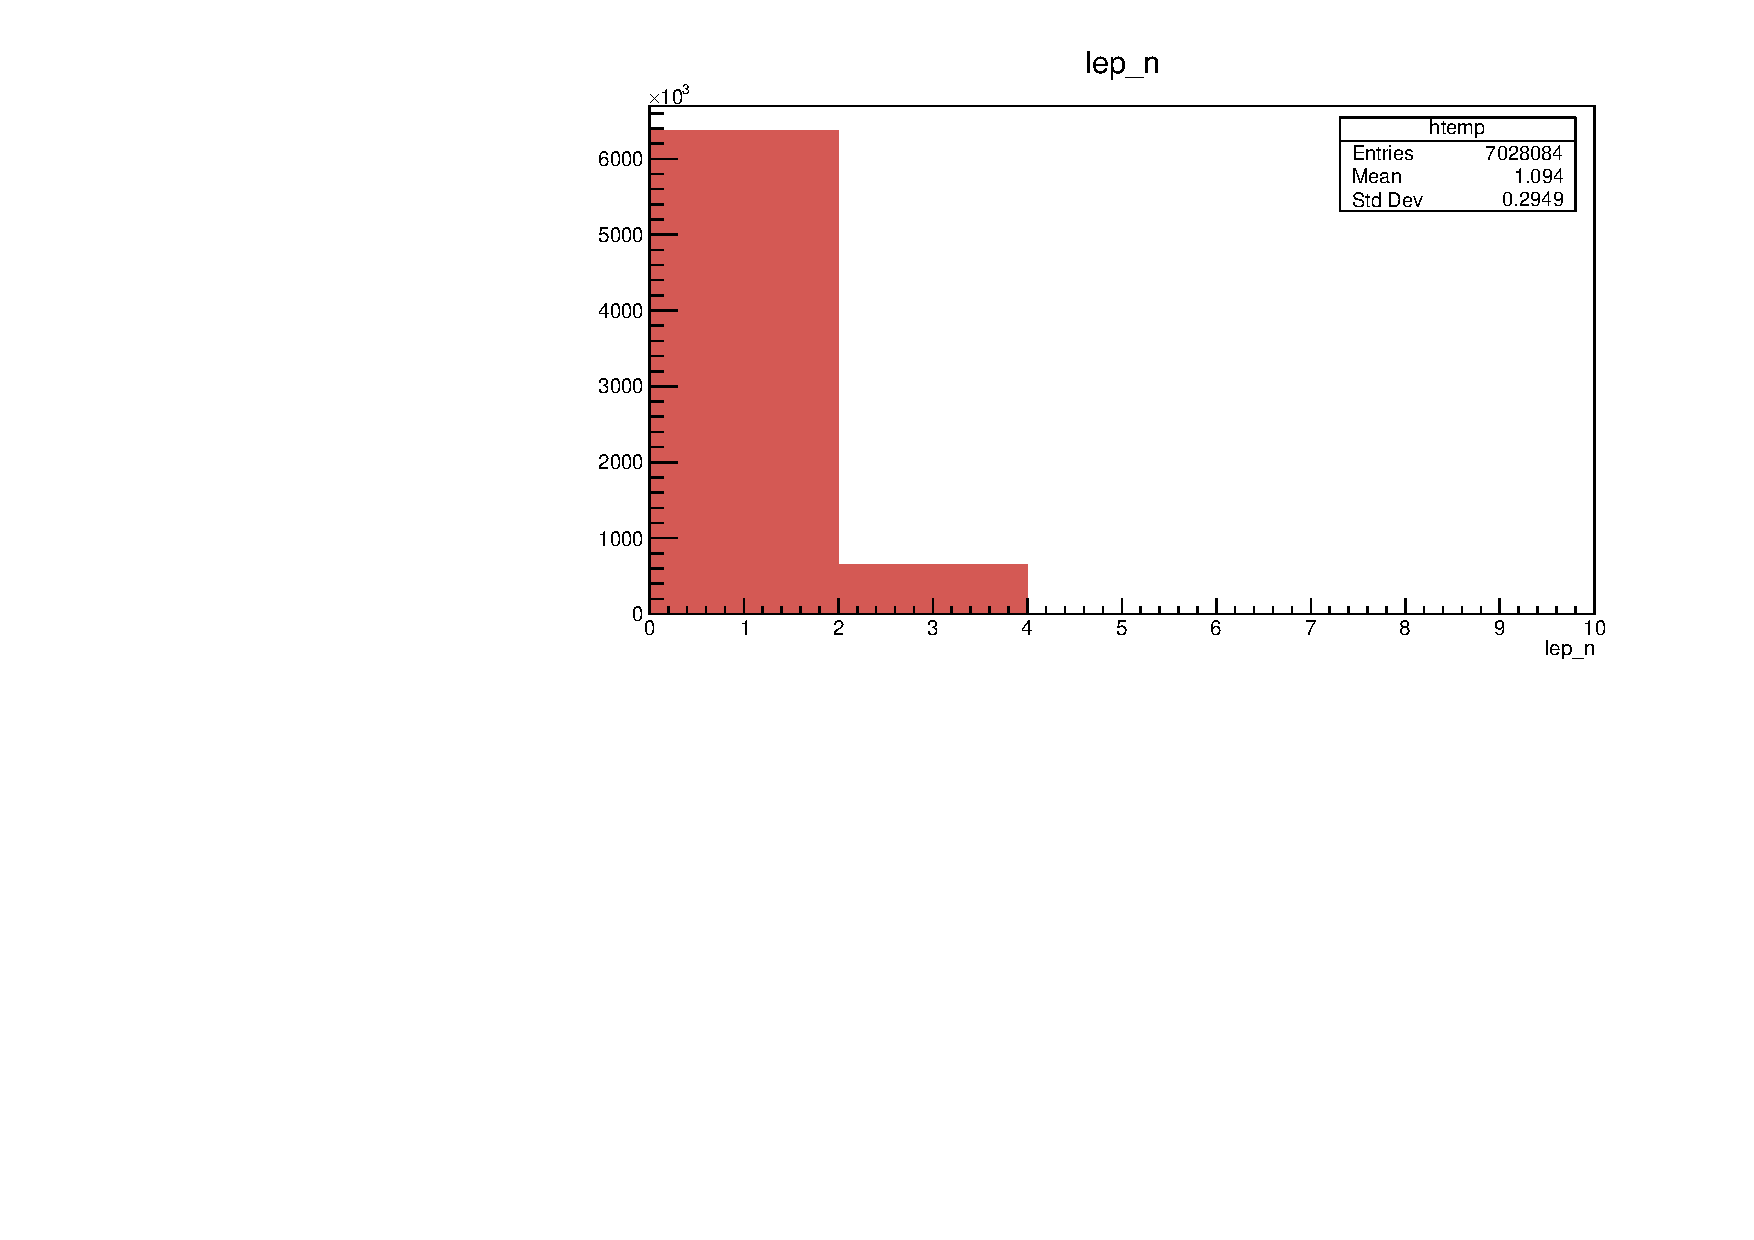
\includegraphics[width=0.45\textwidth]{figures/plots/lep_n_Muons}
	\caption{Number of Leptons in the final state.}
\end{figure}
%TODO: Fix this plot.. 
There are no $Z$ bosons involved in the 1-lepton final state decays and in leading order one would expect two leptons in the final state of the decay process. We are going to take this into account, when setting up our filters.\\

\textbf{Angular and Momentum Distributions.}  
Next we take a look at the distribution of  the pseudorapidity $\eta$, the transversal momentum $p_T$ and its azimutal angle distribution $\phi$.

\begin{figure}[H]
	\centering
	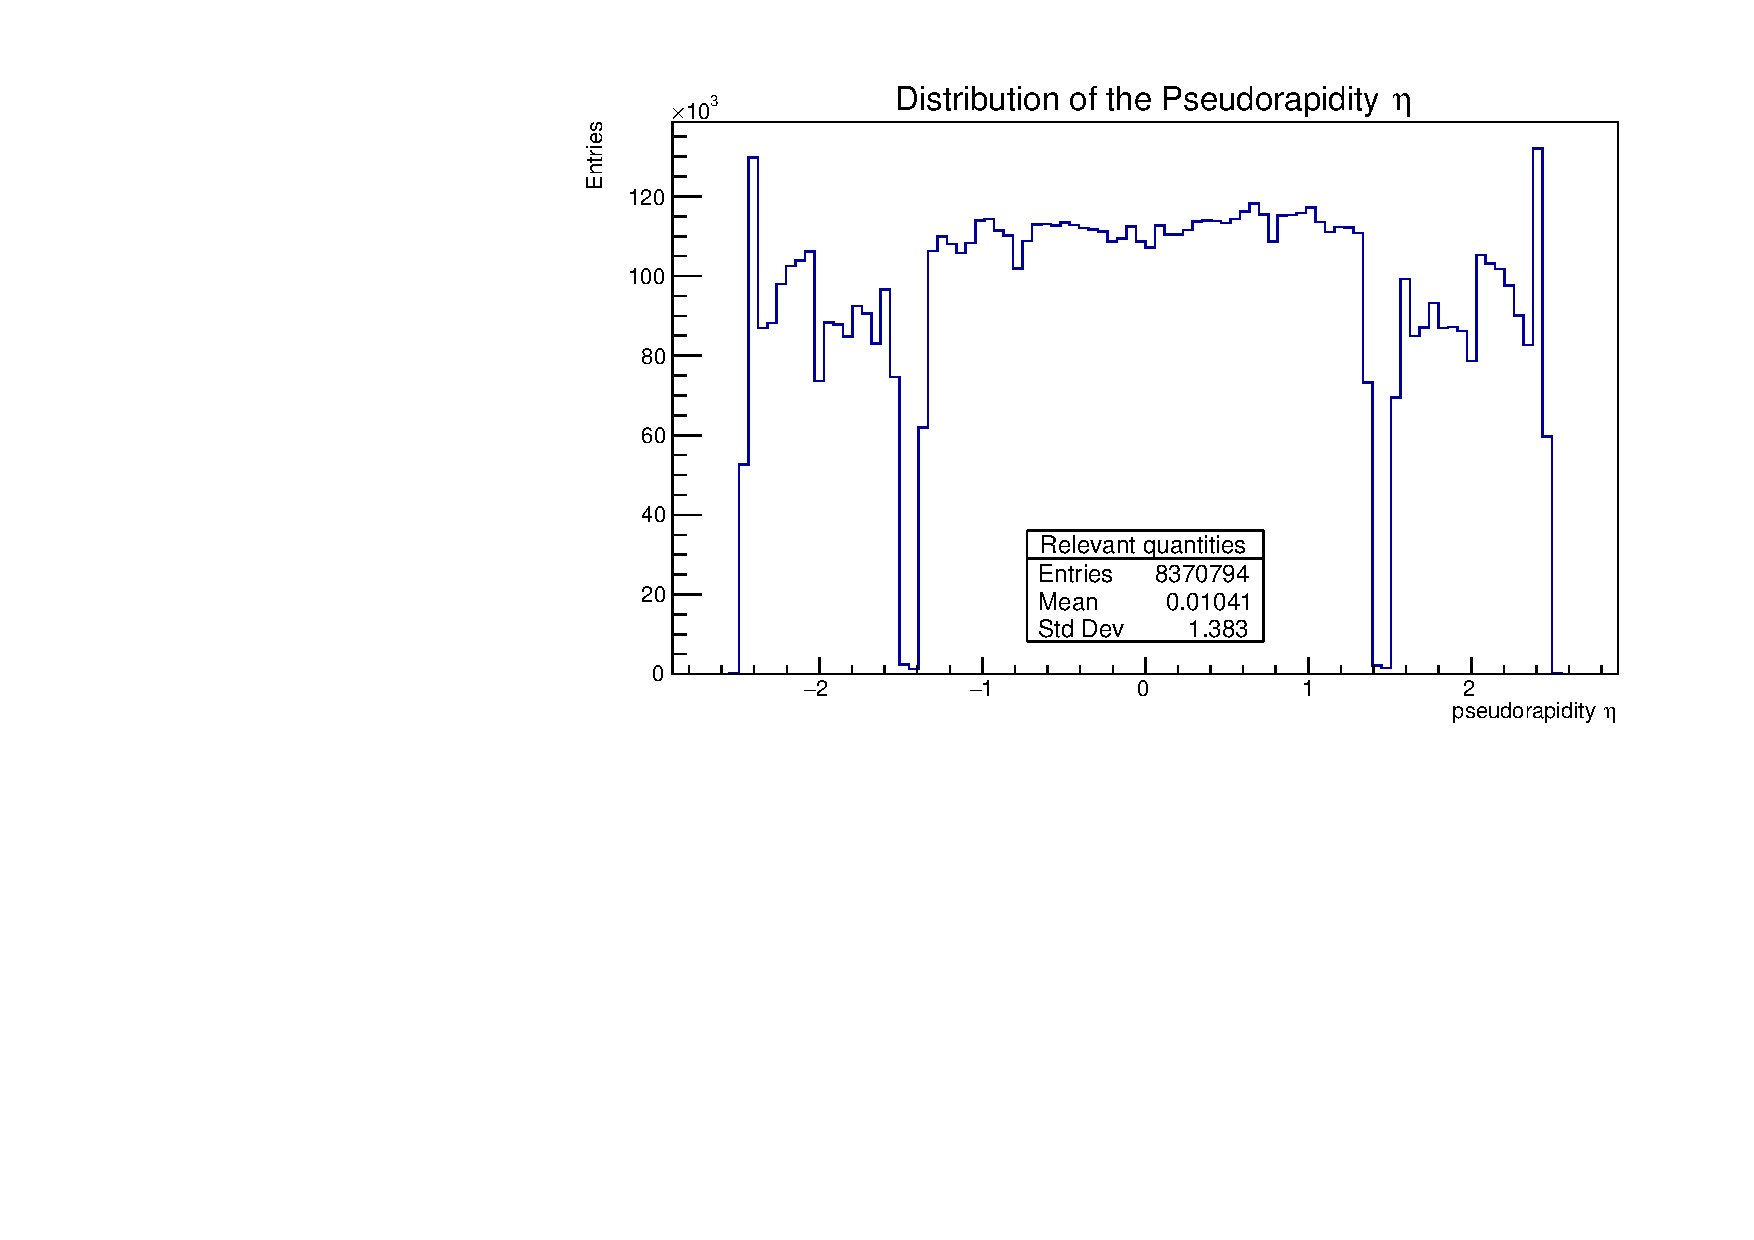
\includegraphics[width=0.45\textwidth]{figures/plots/Pseudorapidity}
	\caption{Distribution of the Pseudorapidity $\eta$.}
\end{figure}

\begin{figure}[H]
	\centering
	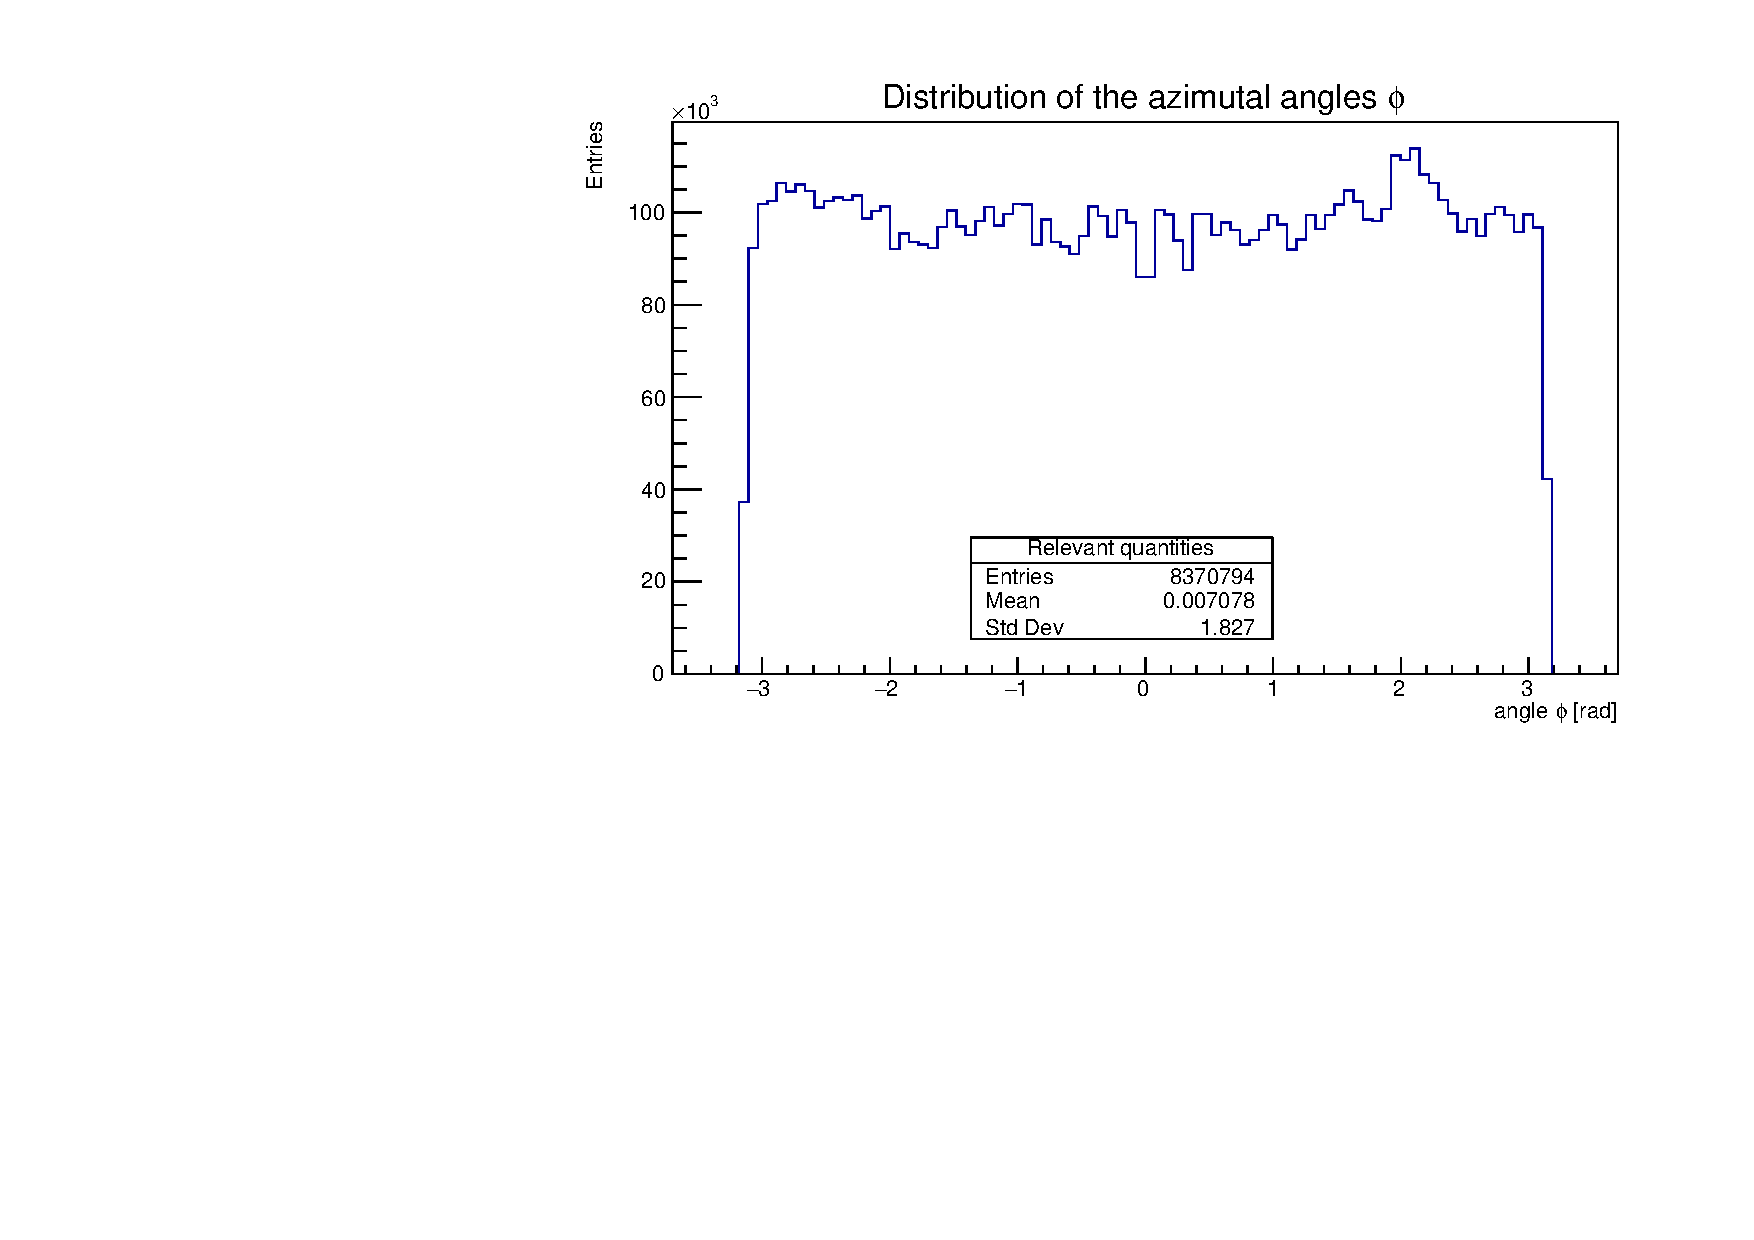
\includegraphics[width=0.45\textwidth]{figures/plots/AzimutalAngle}
	\caption{Distribution of the azimutal angles $\phi$.}
\end{figure}

We would expect, by construction, homogeneously distributed dependencies, but this is only true for $\phi$, while for $\eta$ there are obvious deviations from this.
These can nicely be explained by the geometry of the detector, an explanation that is supported by the symmetry of the stated deviations.\\

The distribution of the transversal momentum shows an unexpected step at about $20$ GeV, caused by the trigger which sorts out all the events where not at least one Lepton has an energy higher than $25$ GeV\footnote{This is useful since there is no way that these events contain a Z-Boson candidate.}.
\begin{figure}[H]
	\centering
	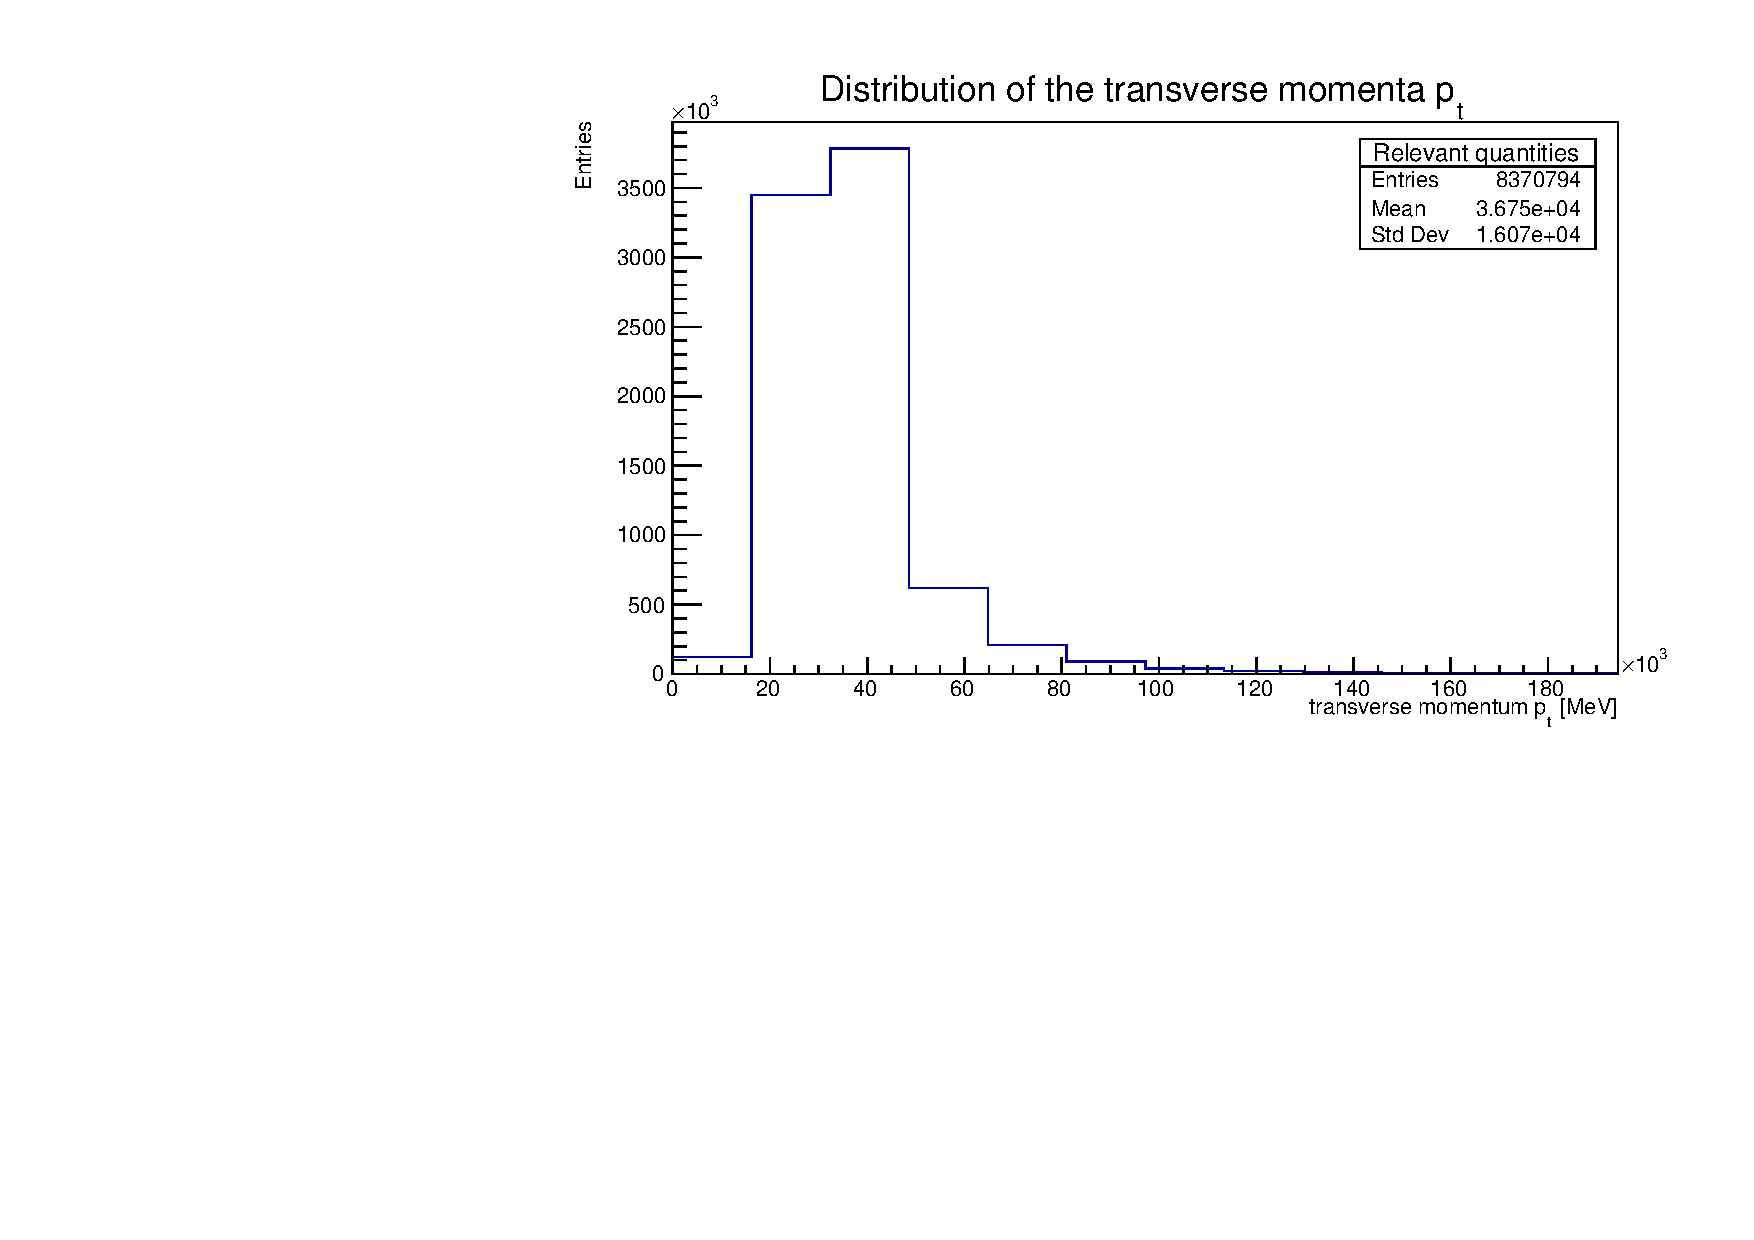
\includegraphics[width=0.45\textwidth]{figures/plots/TransverseMomentum}
	\caption{Distribution of the transverse momenta $p_T$.}
\end{figure}

\subsection{Automating things}
For the next part we adapt the already partially implemented \verb|python| script \verb|eventloop.py| to our needs. New functions for calculating the invariant mass, using \verb|ROOT|'s inbuilt function \verb|TLorenzVector| on the one hand and one by using the theoretical formula $M = \sqrt{E_0^2 - \mathbf{p}^2}$ for the invariant mass on the other hand, are defined. A comparison of both approaches did only show negligible differences that are probably due to truncation errors.\\

Plotting the distribution of the invariant masses in our dataset we could identify several peaks. Their cause is noted on the adjacent plot.
\begin{figure}[H]
	\centering
	\missingfigure{Z spectrum from data}
	\caption{Unfiltered spectrum of the invariant mass distribution for the real dataset.}
\end{figure}

\begin{figure}[H]
	\centering
	\missingfigure{Z spectrum from MC.}
	\caption{Spectrum of the invariant mass distribution for the Monte Carlo distributions.}
\end{figure}
One can clearly see the peak at $90$ GeV, representing the $Z$ boson. There are some other peaks visible in the data, one at $\sim 3$ GeV and the other at $\sim 10$ GeV which correspond to $J/\Psi$ and $\Upsilon$ meson decays. That is the reason why we can't observe such peaks in the Monte Carlo data. Is already mentioned before, there is some sort of peak at around $25$ GeV due to the internal trigger threshold.

\subsection{Selecting events}
To aim for the best possible results, in this part we implemented a series of filters, only leaving the decay processes we could confidently connect to the decay of a Z-Boson.
The following filters were used:
\begin{enumerate}
\item \textbf{Weigths} (for Monte Carlo data only): A measure for the quality of the respective simulation.
\item \textbf{Trigger}: Criteria judging whether it is likely for an event to involve a $Z$ boson decaying into an $e^{+}e^{-}$- or $\mu^{+}\mu^{-}$-pair.
\item \textbf{Vertex}: Is there a comprehensible vertex for the event?
\item \textbf{2 Leptons}: Including only events with exactly two involved leptons.
\item \textbf{PDGID}: This filter is based on the track reconstruction in the detector, which results in an either \textit{loose, medium} or \textit{tight} prediction of the particle type. Every particle type is identified by an integer number (e.\,g. $e = 11 , \ \mu = 13$ and $\tau = 15$).
\item \textbf{$p_T$ Cut}: Do the Leptons have a energy high enough to possibly originate in a $Z$ boson decay?
\item \textbf{Isolation}: Do the Leptons have enough energy to be clearly distinguishable from the background energy of the detector? 
\item \textbf{Tight ID}: Only the particles labelled as \textit{tight} are considered for further analysis.
\item \textbf{$Z$ Mass}: Is the calculated invariant mass anywhere near the theoretical invariant mass of a $Z$ boson?
\end{enumerate}

After applying all the filters to the data we can plot the amount of measurements that passed the tests until a certain  filter. This kind of diagram is called \textit{Cut Flow diagram}. For our filter setting, the Cut Flow diagram is depicted in the following.
%TODO: Include OUR Cut Flow Diagram
\begin{figure}[H]
\centering
\includegraphics[width = 0.5\textwidth]
{figures/plots/CutFlowEGamma}
\caption{Cut flow diagram for our event selection algorithm applied to the EGamma dataset.}	
\end{figure}


In order to be able to compare the data to the theoretical predictions, we analyze Monte Carlo simulations of $Z$ boson decays into $e^+e^-$-, $\mu^+\mu^-$- and $\tau^+\tau^-$-pairs, represented in the following (stacked) diagram: %(\ref{fig:MChisto}) 

\begin{figure}[H]
	\centering
	\missingfigure{Stacked MC data histogram.}
	\caption{Results for Monte Carlo simulations of $Z$-boson decays into $e^+e^-$-, $\mu^+\mu^-$- and $\tau^+\tau^-$-pairs.}
	\label{fig:MChisto}
\end{figure}

For a more realistic comparison, we need to rescale the data to match them to the real parameters from the measurements. We use the formula $k = \sfrac{\mathcal{L}\sigma}{w}$, where $w$ represents the MC weight we introduced above. In practice, the scaling is implemented directly in the \verb|Python| script, which means there is no warranty at all that the scaling is set optimally. \\

%TODO: Short comment on the plots..
\blindtext
\section{Fitting the $Z$ mass}

We want to use this section to present the final result for the mass distribution of the processes with $Z$-candidates which passed all filter levels. The result is presented in the following in figure (\ref{fig:MassDist}).

\begin{figure}[H]
	\centering
	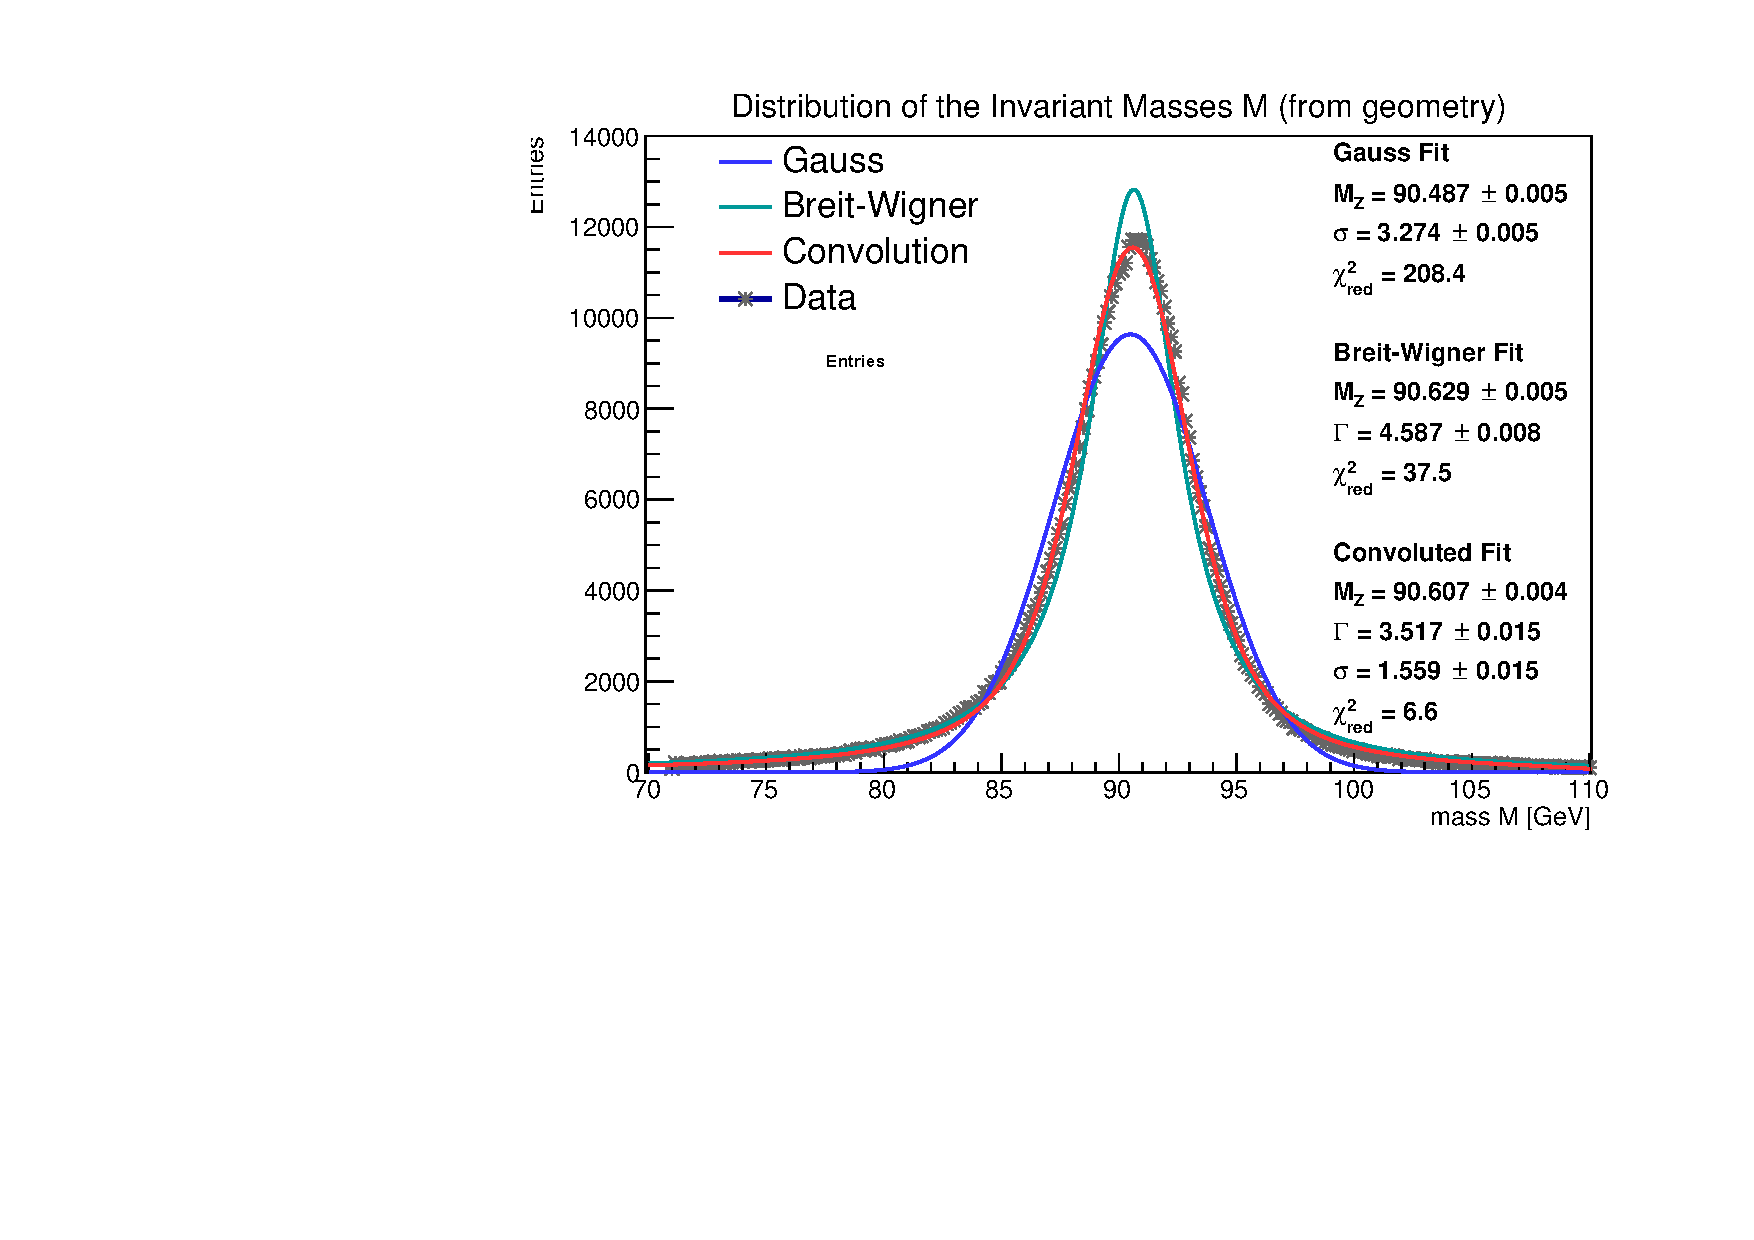
\includegraphics[width = 0.45\textwidth]{figures/plots/ZMassFitted}
	\caption{Distribution of the $Z$ masses $M_{\mathrm{Z}}$ with Gaussian, Breit-Wigner and a convoluted fit.}
	\label{fig:MassDist}
\end{figure}

As discussed before, to obtain a satisfying fitting result one needs to convolute a Breit-Wigner distribution and a Gaussian. We can directly see in figure (\ref{fig:MassDist}), that the fits using the two functions separately did not represent the physical model in an adequate manner.
The results from the convoluted fit are the following. \\

For the mass of the $Z$ boson we found
\begin{align}
	M_{\mathrm{Z}} = (90.607 \pm 0.004) \ \text{GeV},
\end{align} 
the decay width $\Gamma$ is
\begin{align}
\Gamma = (3.517 \pm 0.015) \ \text{GeV},	
\end{align}
and the the Gaussian we used to describe the smearing of the distribution due to the measurement process has a standard deviation of 
\begin{align}
	\sigma = (1.559 \pm 0.015) \ \text{GeV}.
\end{align}

These results can be compared to the values of the Particle Data Group\footnote{The values can be found here: \url{http://pdg.lbl.gov/2018/listings/rpp2018-list-z-boson.pdf}} (PDG), 
\begin{align}
	M_{\mathrm{Z}}&=(91.1876 \pm 0.0021) \ \mathrm{GeV} \\  \nonumber\\ \Gamma&=(2.4952 \pm 0.0023) \ \mathrm{GeV}.
\end{align} 
Using Gaussian error propagation one finds for the differences between our final results and the PDG data
\begin{align}
	\Delta M_{\mathrm{Z}}&=(0.581 \pm 0.005) \ \mathrm{GeV} \\  \nonumber\\ 
	\Delta\Gamma&=(1.022 \pm 0.015) \ \mathrm{GeV},
\end{align} 
which means the deviations are approximately of order $\sim$ 1 GeV. The errors seem to be very small, which is explained by the fact, that all errors we take into account at the moment only come from the fitting process. This is presumeably a highly underestimating treatment of errors. We'll come back to this during the critical discussion of the results in the next section.
\section{Critical discussion}
In this section we want to discuss the role of the systematic and statistical errors and their possible influence on our results.\\

The data set we analyzed is very large, this means we had enough measurements to reduce statistical uncertainties to a negligible minimum. We know from Poisson statistics, that the significance of the corresponding errors can be estimated using the inverse square root of the amount of data. In total this means that it should hold, that $\Delta_{\mathrm{stat.}} \ll \Delta_{\mathrm{syst.}}$. \\
A measure for the possible influence of the systematical uncertainties is given by the standard deviation \\ $\sigma = (1.559 \pm 0.015) \ \text{GeV}$ we concluded from the convoluted fit. It clearly shows that one has to keep in mind that the energy resolution inside the calorimeter is not perfect. In general one has to think about the treshold values for the filter system. When we would have had additional time, we could have tested the impact of changes in the different steps of the implemented filter.
%TODO: Some more on syst. errors?

\section{Conclusion}
After some preparation time to be able to understand the underlaying structure of the analyzed dataset, the main goal of this lab course was to get familiar with modern data analysis tools such as \verb|ROOT| and \verb|Python| and to handle a large amount of data, by implementing our own multi-level filter system, to be able to distinguish possible $Z$ boson candidates from other measurements. We also had the chance to compare the data to theoretical predictions by analyzing some Monte Carlo simulations. Our final result for the $Z$ mass and its decay width $\Gamma$ seem to fit to the values provided by the PDG. Only the treatment of, especially the systematic error sources,  has to  be questioned, as we did in the previous section. Nevertheless we can conclude, that the obtained results are compatible with the expectations.\\
We can remark, that we learned a lot about data-analysis in particle and we had a lot of fun implementing the filters.  
\begin{acknowledgments}
We would like to thank our supervisor Philipp Ott for his guidance throughout the operation of this experiment.
\end{acknowledgments}

\bibliographystyle{abbrv}
\bibliography{bibliography/literatur}
\nocite{*}

\end{document}
